% \documentclass{standalone}
% \usepackage{tikz}
% \usetikzlibrary{patterns}
% \begin{document}
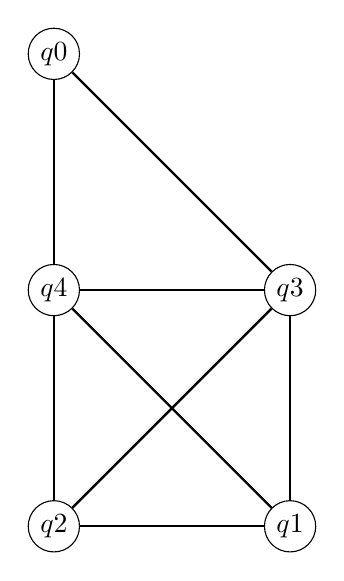
\begin{tikzpicture}
    \definecolor{lightgray}{rgb}{0.8,0.8,0.8}
    \definecolor{darkgreen}{rgb}{0  ,0.5,0  }
    \tikzset{
        unuseNode/.style={
            circle,
            draw=blue,
            dashed, % Dashed outline
            % fill=red, % Solid fill color
            % pattern=vertical lines, % Pattern type
            minimum size=12pt,
            inner sep=0pt
        },
        useNode/.style={circle, draw=black, minimum size=8pt, inner sep=2pt},
        fontNode1/.style={above right, font=\Large },
        fontNode2/.style={right, midway,font=\small}
    }


    % \node[useNode] (q0) at (0,6) {};
    % \node[fontNode1] at (q0) {$q0$};
    % \node[useNode] (q1) at (3,0) {};
    % \node[fontNode1] at (q1) {$q1$};
    % \node[useNode] (q2) at (0,0) {};
    % \node[fontNode1] at (q2) {$q2$};
    % \node[useNode] (q3) at (3,3) {};
    % \node[fontNode1] at (q3) {$q3$};
    % \node[useNode] (q4) at (0,3) {};
    % \node[fontNode1] at (q4) {$q4$};
    \node[useNode] (q0) at (0,6) {$q0$};
    \node[useNode] (q1) at (3,0) {$q1$};
    \node[useNode] (q2) at (0,0) {$q2$};
    \node[useNode] (q3) at (3,3) {$q3$};
    \node[useNode] (q4) at (0,3) {$q4$};

    \draw[-,line width = 0.3mm] (q0) -- (q4) node[fontNode2] {};
    \draw[-,line width = 0.3mm] (q0) -- (q3) node[fontNode2] {};
    \draw[-,line width = 0.3mm] (q4) -- (q3) node[fontNode2] {};
    \draw[-,line width = 0.3mm] (q4) -- (q2) node[fontNode2] {};
    \draw[-,line width = 0.3mm] (q4) -- (q1) node[fontNode2] {};
    \draw[-,line width = 0.3mm] (q3) -- (q2) node[fontNode2] {};
    \draw[-,line width = 0.3mm] (q1) -- (q3) node[fontNode2] {};
    \draw[-,line width = 0.3mm] (q1) -- (q2) node[fontNode2] {};
\end{tikzpicture}
% \end{document}
